
\newcommand{\note}[1]{\begin{ccTexOnly}%
{\color{red}$\langle\!\langle$#1$\rangle\!\rangle$}\end{ccTexOnly}}
\newcommand{\sphere}{\ensuremath{\mathcal S}}
\renewcommand{\real}{\ensuremath{\mathbb R}}

This package proposes data structure and algorithms to compute
triangulations of points in any dimensions.
The \ccc{Triangulation_data_structure} allows to store and manipulate the
combinatorial part of a triangulation while the geometric classes
\ccc{Triangulation} and \ccc{Delaunay_triangulation} allows to
compute a (Delaunay) triangulation of a set of points and to maintain
it under insertions (and deletions in the Delaunay case).


\section{Introduction\label{triangulation:intro}}

\subsubsection{Some definitions}

A {\em finite abstract simplicial complex} is built on a finite set of
vertices $V$ and consists of a collection $S$ of subsets of $V$ such that

\centerline{if $s$ is a set of vertices in $S$, then all the subsets of $s$ are also
in $S$.}

The sets in $S$ (which are subsets of $V$) are called
{\em faces} or {\em simplices} (the
singular of which is {\em simplex}).
%
A simplex $s\in S$ is {\em maximal} if it is not a proper subset of some other
set in $S$. The simplicial complex is {\em pure} %(or {\em homogeneous})
if all the maximal simplices have the same cardinality, i.e., they have the same
number of vertices.
In the sequel, we will call these maximal simplices {\em full cells}.
A {\em face} of a simplex is a subset of it.
A {\em proper face} of a simplex is a strict subset of it.

If the vertices are embedded into Euclidean space $\real^d$, we deal with
{\em finite simplicial complexes} which have slightly different simplices
and additional requirements:
\begin{itemize}
\item vertices corresponds to points in space.
\item a simplex $s\in S$ is the convex hull of its vertices.
\item the vertices of a simplex $s\in S$ are affinely independent.
\item the intersection of any two simplices of $S$ is a proper face of both
simplices (the empty set counts).
\end{itemize}
See the \ccAnchor{http://en.wikipedia.org/wiki/Simplicial_complex}{wikipedia
entry} for more about simplicial complexes.

\subsubsection{What's in this package?}

This \cgal\ package deals with pure finite simplicial complexes
without boundary, which
we will simply call in the sequel {\em triangulations}. It provides three main classes
for creating and manipulating triangulations.

The class \ccc{CGAL::Triangulation_data_structure<Dimensionality,
TriangulationDSVertex, TriangulationDSFullCell>} models an {\em abstract triangulation}: vertices in this
class are not embedded in Euclidean space but are only of combinatorial
nature.

The class \ccc{CGAL::Triangulation<TriangulationTraits, TriangulationDataStructure>} embeds an abstract
triangulation in Euclidean space, thus forming a geometric
triangulation. Methods are
provided for the insertion %and removal
of points in the triangulation, the
traversal of various elements of the triangulation, as well as the localization of a
query point inside the triangulation.
The convex hull of the points is part of the triangulation, the fact
that there is no boundary is ensured by adding an infinite vertex and
infinite full cells to triangulate the outside of the convex hull.

The class \ccc{CGAL::Delaunay_triangulation<DelaunayTriangulationTraits, TriangulationDataStructure>} adds further
constraints to a triangulation, in that all its simplices must have the
so-called {\em Delaunay} or {\em empty-ball} property: the interior of
a ball circumscribing any simplex (or full cell) must be free from any
vertex of the triangulation. The \ccc{CGAL::Delaunay_triangulation} class
supports deletion of vertices.

%The class \ccc{CGAL::Regular_triangulation<RegularTraits, TriangulationDataStructure>} is a generalization of
%the Delaunay triangulation.

%The rest of this user manual gives more details about these classes and the
%data they store, but does not tell the whole story. For the latter, the user
%should have a look at the reference manual of this package.

%A last remark:
%pure complexes are also called \emph{triangulations}. We feel more confortable
%in using the word \emph{complexes} as it forces us to think ``in dimension
%higher than 3''.

\subsubsection{Further definitions}

An $i$-face denotes an $i$-dimensional simplex, or a simplex with $i+1$
vertices. When these vertices are embedded in Euclidean space, they must be
affinely independent.

If the maximal dimension of a simplex in the triangulation is
$d$, we call:\begin{itemize}
\item an $i$-face for some $i\in[0,d]$ a  {\em face};
\item a $0$-face a {\em vertex};
\item a $1$-face an {\em edge};
\item a $(d-2)$-face a {\em ridge};
\item a $(d-1)$-face a {\em facet}; and
\item a $d$-face  a {\em full cell}.
\end{itemize}

Two faces $\sigma$ and $\sigma'$ are {\em incident} if and only if
$\sigma'$ is a proper sub-face of $\sigma$ or \emph{vice versa}.

\section{Triangulation Data Structure\label{triangulation:tds}}

\newcommand{\tds}{\ccc{TriangulationDataStructure}}
\newcommand{\ad}{\ensuremath{D}}
\newcommand{\cd}{\ensuremath{d}}

In this section, we describe the concept \ccc{TriangulationDataStructure} for
which \cgal\ provides one model class:
\ccc{CGAL::Triangulation_data_structure<Dimensionality, TriangulationDSVertex,
TriangulationDSFullCell>}.%  For simplicity, we use the abbreviation \tds.

A \tds\ can represent an abstract pure complex
such that any facet is incident to exactly two full cells.

A \tds\ has a property called the {\em maximal dimension} which is a
positive integer equal to the maximum dimension a full cell can have.
This maximal dimension can be chosen by the user at the creation of a \tds\
and can then be queried using the method \ccc{tds.maximal_dimension()}.
A \tds\ also knows the {\em current dimension} of its full cells,
which can be queried with \ccc{tds.current_dimension()}. In the sequel, let
us denote the maximal dimension with \ad\ and the current dimension with \cd.
The inequalities $-2\leq\cd\leq\ad$ and $0<\ad$ always hold.
The special meaning of negative values for $d$ is explained below.

%\note{I remove some comments about 3D vs dD which are not exact. %
%in T3D package in degenerate dimension \ccc{Cell} is actually used with the %
%same meaning as here (a $d$-face  and not a $D$-face).}
%% \paragraph{On the \ccc{Facet} nested type}
%%  In the \ccc{Triangulation_3} \cgal\ package, the maximal dimension is always
%% 3. With respect to this reference dimension (3), a \ccc{Facet} is always a
%% 2-face (triangle),
%% irrespective of the 3D triangulation's current dimension. In
%% particular, full cells in degenerate planar 3D triangulation are
%% \ccc{Facet}s, not \ccc{Cell}s.
%
%% By contrast, in the present \ccc{Triangulation} \cgal\ package, the reference
%% dimension of a pure complex (or a pure complex data structure) is its current
%% dimension. This means that, whatever the current dimension is, a
%% full cell is always represented by the \ccc{FullCell} nested type, And a
%% \ccc{Facet} represents a face of dimension \ccc{current_dimension()-1}
%% {\em and not} \ccc{maximal_dimension()-1}.

\subsubsection{The data structure triangulates $\sphere^\cd$}

A \tds\ can be viewed as
a {triangulation} of the topological sphere $\sphere^\cd$,
i.e., its faces can be embedded to form a partition of
$\sphere^\cd$ into $\cd$-simplices.
% When a
% \tds\ is used as the combinatorial part of a geometric triangulation, one
% special vertex of the \tds\ plays the role of the {\em vertex at
% infinity}; we can consider that the triangulation covers the whole
% affine hull of its vertices
% using {\em infinite} or {\em unbounded} full cells to fill the space  outside the convex
% hull of the triangulation's finite vertices. (More details are given in the next section.)


One nice consequence of the above important fact is that a full cell has
always exactly  $\cd+1$ neighbors.
Two  full cells $\sigma$ and $\sigma'$ sharing a facet are called
{\em neighbors}.

\newcommand{\cgalTriangulationCurrentDimension}{%
\item[$\cd=-2$] This corresponds to the non-existence of any object in
        the \tds.
    \item[$\cd=-1$] This corresponds to a single vertex and a single full cell. In a
        geometric triangulation, this vertex corresponds to the vertex at infinity.
    \item[$\cd=0$] This corresponds to two vertices (geometrically, the finite vertex and
        the infinite vertex), each corresponding to  a full cell;
        the two full cells being neighbors of each other. This is the unique
        triangulation of the $0$-sphere.
    \item[$0<\cd\le\ad$] This corresponds to a standard triangulation of
        the sphere $\sphere^\cd$.}

Possible values of $\cd$ (the \emph{current dimension} of the triangulation) include
%\begin{ccTexOnly}
%    \begin{list}{}{\leftmargin=20mm\labelsep=3mm\labelwidth=17mm}
%    \cgalTriangulationCurrentDimension
%    \end{list}
%\end{ccTexOnly}
%\begin{ccHtmlOnly}
\begin{quotation}
    \noindent\begin{itemize}
    \cgalTriangulationCurrentDimension
    \end{itemize}
\end{quotation}
%\end{ccHtmlOnly}

% - - - - - - - - - - - - - - - - - - - - - - - - - - - - T D S IMPLEMENTATION

\subsection{The class \ccc{Triangulation_data_structure}\label{triangulation:tds:impl}}

We give here some details about the class
\ccc{Triangulation_data_structure<Dimensionality, TriangulationDSVertex,
TriangulationDSFullCell>}
implementing the concept \ccc{TriangulationDataStructure}.


\subsubsection{Storage}

A \tds\ explicitly stores its vertices and full cells.

Each vertex stores a reference (a \ccc{handle}) to one of its incident
full cells.


Each full cell stores references to its $\cd+1$ vertices and
neighbors. Its vertices and neighbors are indexed from $0$ to \cd. The indices
of its neighbors have the following meaning: the $i$-th neighbor of $\sigma$
is the unique neighbor of $\sigma$ that does not contain the $i$-th vertex of
$\sigma$; in other words, it is the neighbor of $\sigma$ {\em opposite} to
the $i$-th vertex of $\sigma$ (Figure~\ref{triangulation:fig:full-cell}).

\begin{figure}[htbp]
\begin{ccTexOnly}
\begin{center}
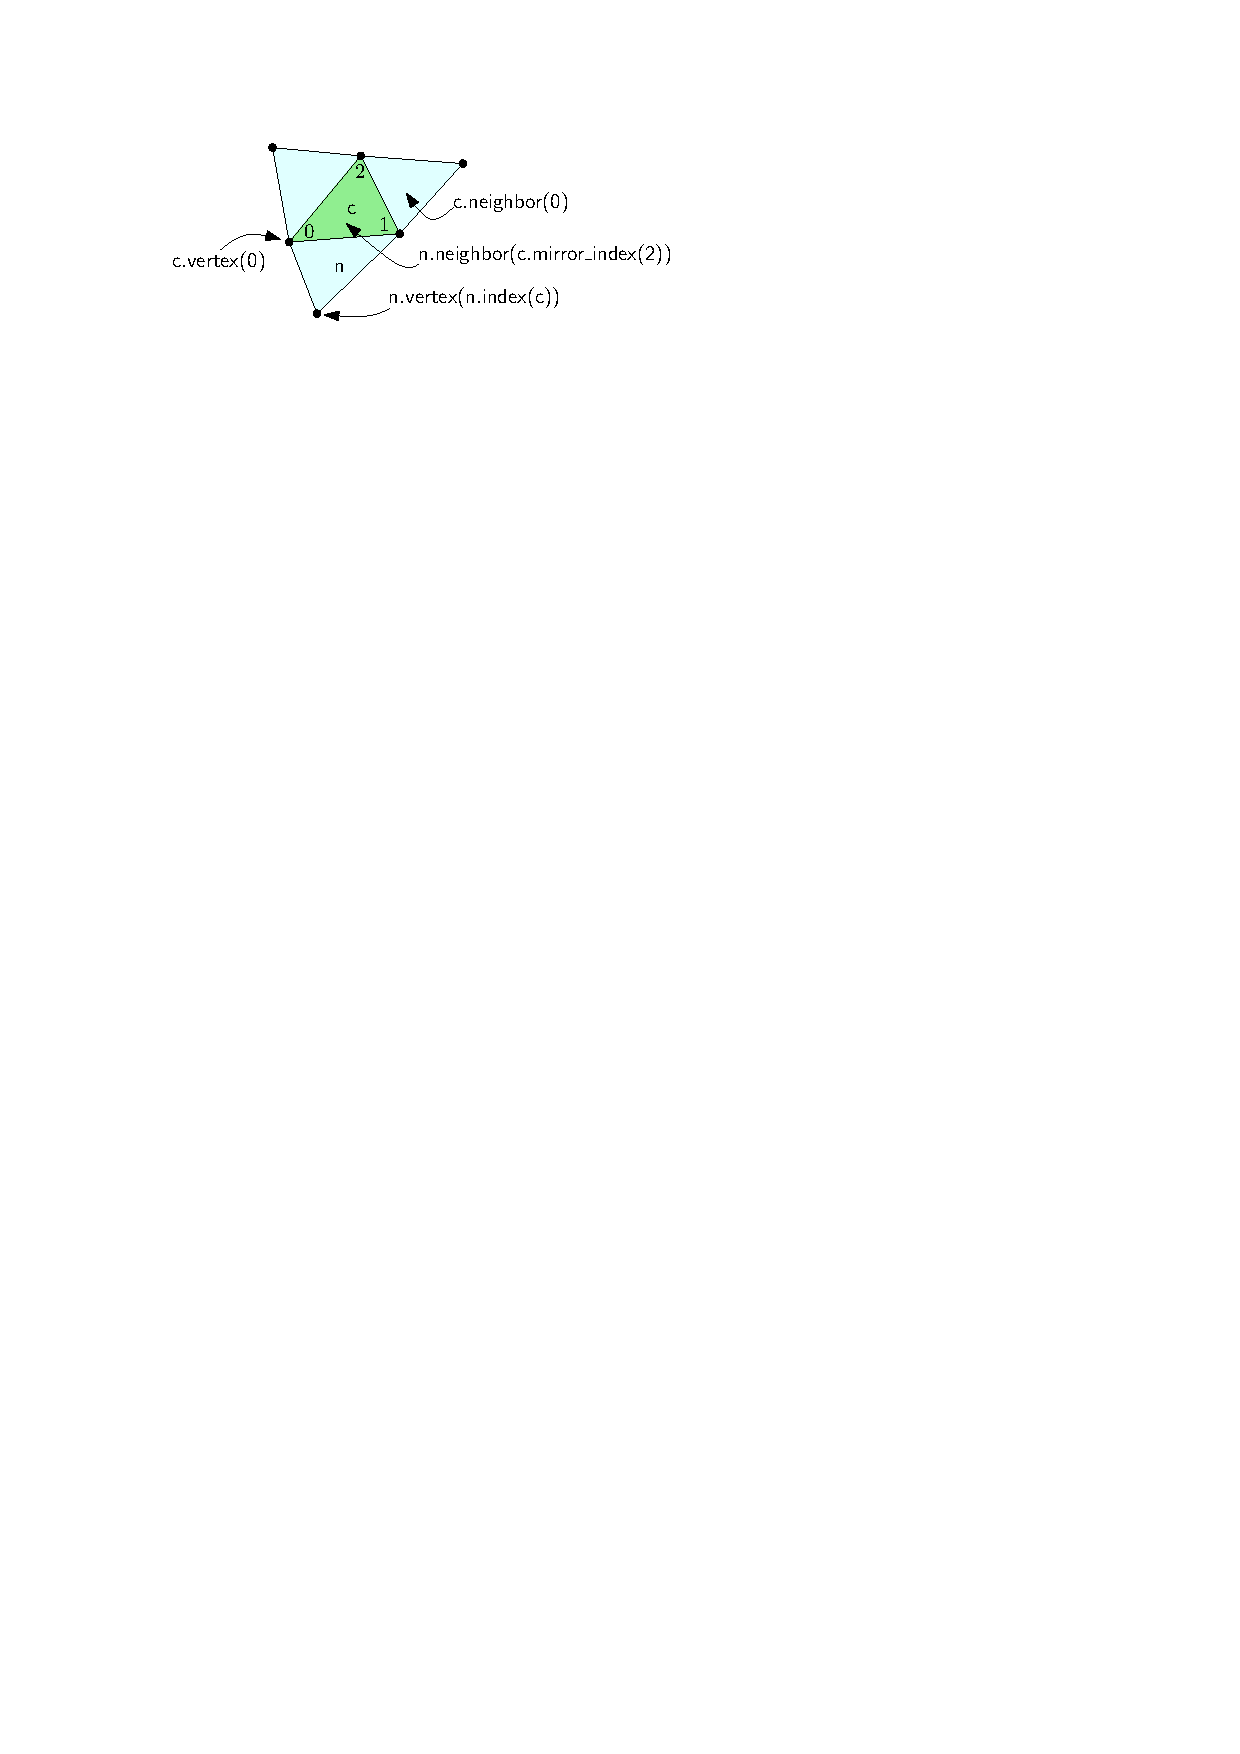
\includegraphics{Triangulation/fig/simplex-structure.pdf}
\end{center}
\end{ccTexOnly}
\begin{ccHtmlOnly}
<center>
<img border=0 src="./fig/simplex-structure.png" align="middle"
alt="Index the vertices and neighbors of a full cell">
</center>
\end{ccHtmlOnly}
\caption{Indexing the vertices and neighbors of a full cell $c$ in
  dimension $\cd=2$.}
\label{triangulation:fig:full-cell}
\end{figure}

\begin{ccAdvanced}
The index of a full cell $c$ in the $i$-th neighbor of $c$ is called the
\emph{$i$-th mirror-index} of $c$ (Figure~\ref{triangulation:fig:full-cell}).
Mirror indices are often needed for maintaining the triangulation data
structure. Thus, it might be desirable, for performance reasons, to store the
mirror indices alongside the references to the vertices and neighbors in a full
cell. This improves speed a little, but requires more memory.

\cgal\ provides the class template
\ccc{Triangulation_ds_full_cell<TriangulationDataStructure,
TDSFullCellStoragePolicy>} for representing full cells in a triangulation. Its
second template parameter is used to specify wether or not the mirror indices
should be kept in memory or computed on-the-fly, which is the default case.
Please refer to the documentation of that class template for specific details.
\end{ccAdvanced}

\subsubsection{Instantiating the class template}

The \ccc{Triangulation_data_structure<Dimensionality, TriangulationDSVertex, TriangulationDSFullCell>}
class template is designed in such a way that its user can choose
\begin{itemize}
\item the maximal dimension of the triangulation data structure by specifying the \ccc{Dimensionality} template parameter,
\item the type used to represent vertices by specifying the \ccc{TriangulationDSVertex}
template parameter and
\item the type used to represent full cells by specifying the
\ccc{TriangulationDSFullCell} template parameter.
\end{itemize}

The last two parameters have default values and are thus not necessary, unless
the user needs custom types (see the reference manual page for this class
template). The first template parameter, \ccc{Dimensionality}, must be
one of the following:
\begin{itemize}
\item \ccPureGlobalScope\ccc{Dimension_tag<D>} for some integer \ad. This
indicates that the triangulation can store full cells of dimension at most
\ad. The maximum dimension \ad\ is known by the compiler, which
triggers some optimizations.
\item \ccPureGlobalScope\ccc{Dynamic_dimension_tag}. In this case, the maximum
dimension of the full cells must be passed as an integer argument to an instance
constructor (see \ccc{TriangulationDataStructure}).
\end{itemize}

The \ccc{TriangulationDSVertex} and \ccc{TriangulationDSFullCell} parameters to the class template
must be models of the concepts \ccc{TriangulationDSVertex} and
\ccc{TriangulationDSFullCell} respectively. \cgal\ provides models for these
concepts: \ccc{Triangulation_ds_vertex<TriangulationDataStructure>} and
\ccc{Triangulation_ds_full_cell<TriangulationDataStructure, TDSFullCellStoragePolicy>}, which, as one
can see, take the \tds\ as a template parameter in order to get access to
some nested types in \tds.

{\em This creates a circular dependency}, which we resolve in the same way
as in the \cgal\ \ccc{Triangulation_2} and \ccc{Triangulation_3} packages (see
Chapters~\ref{chapter-TDS2},~\ref{chapter-Triangulation2},~\ref{chapter-TDS3},~and~\ref{chapter-Triangulation3}).
In particular, models of the concepts \ccc{TriangulationDSVertex} and
\ccc{TriangulationDSFullCell} must provide a nested template \ccc{Rebind_TDS}
which is documented in those two concept's reference manual pages.

\begin{ccAdvanced}
The user that is in need of a custom vertex or full cell class, is
encouraged to read the documentation of the \cgal\
\ccc{Triangulation_2}  or  \ccc{Triangulation_3} package.
\end{ccAdvanced}

% - - - - - - - - - - - - - - - - - - - - - - - - - - - - - - TDS EXAMPLES

\subsection{Examples\label{triangulation:tds:examples}}

\subsubsection{Incremental Construction}
The following examples shows how to construct a triangulation data structure by
inserting vertices. Its main interest is that it demonstrates most of the API
to insert new vertices into the triangulation. Therefore, the reader will make
the best use of this example by reading it slowly, together with the reference
manual documentation of the methods that are called (see here:
\ccc{TriangulationDataStructure}) and by trying to understand the various
\ccc{assert(...)} statements.

\ccIncludeExampleCode{Triangulation/triangulation_data_structure_static.cpp}

In previous example, the maximal dimension is fixed at compile time.
It is also possible to fix it at run time, as in the next example.

\ccIncludeExampleCode{Triangulation/triangulation_data_structure_dynamic.cpp}

\subsubsection{Barycentric subdivision}
This example provides a function for computing the barycentric subdivision of a
single full cell \ccc{c} in a triangulation data structure. The other
full cells adjacent to \ccc{c} are automatically subdivided to match the
subdivision of the full cell \ccc{c}. The barycentric subdivision of \ccc{c} is
obtained by enumerating all the faces of \ccc{c} in order of decreasing
dimension, from the dimension of~\ccc{c} to dimension~1, and inserting a new
vertex in each face. For the enumeration, we use a combination enumerator,
which is not documented, but provided in \cgal.


\begin{figure}[htbp]
\begin{ccTexOnly}
\begin{center}
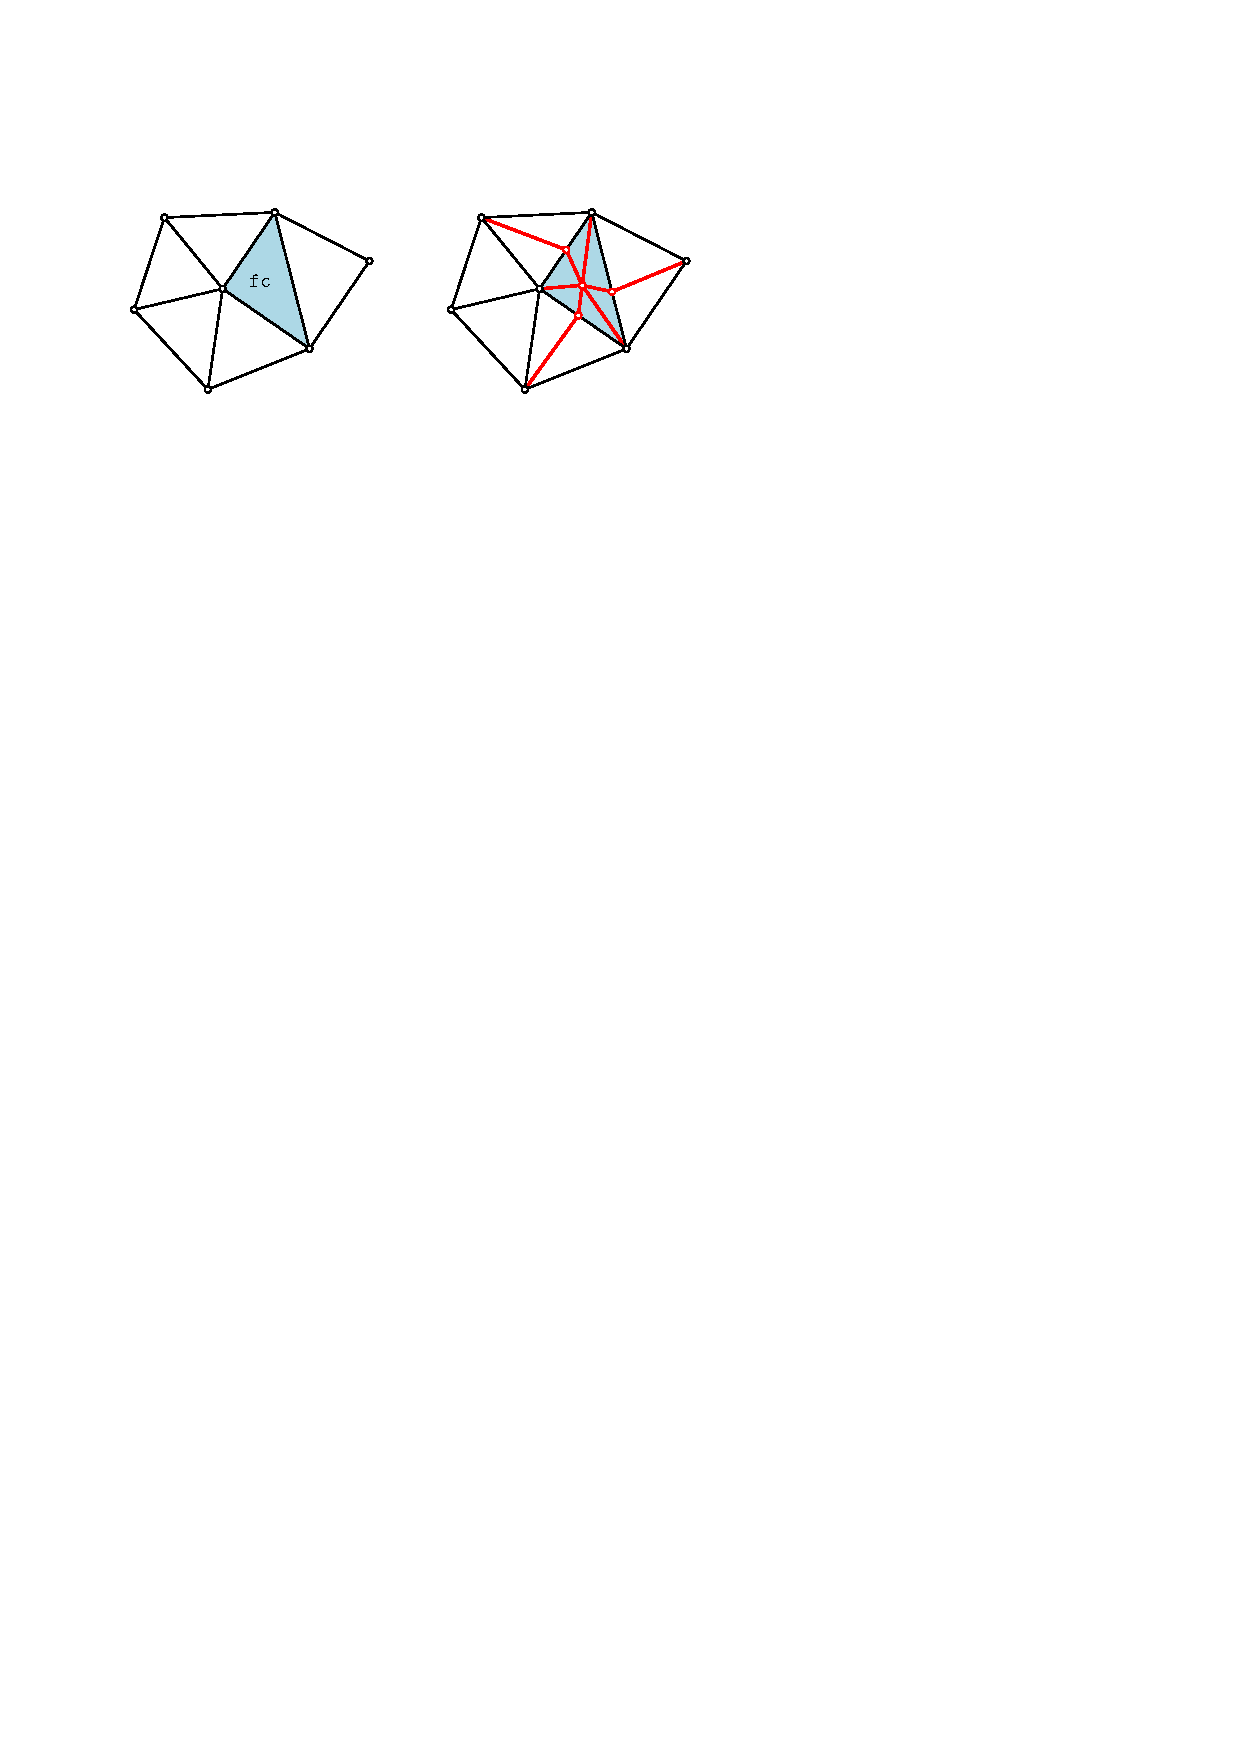
\includegraphics{Triangulation/fig/barycentric-subdivision.pdf}
\end{center}
\end{ccTexOnly}
\begin{ccHtmlOnly}
<center>
<img border=0 src="./fig/barycentric-subdivision.png" align="middle"
alt="Barycentric subdivision">
</center>
\end{ccHtmlOnly}
\caption{Barycentric subdivision in  dimension $\cd=2$.}
\label{triangulation:fig:barycentric}
\end{figure}

\ccIncludeExampleCode{Triangulation/barycentric_subdivision.cpp}


% - - - - - - - - - - - - - - - - - - - - - - - - - - - - - - TRIANGULATIONS

\section{Triangulations}

The class \ccc{CGAL::Triangulation<TriangulationTraits, TriangulationDataStructure>} embeds an abstract
triangulation into Euclidean space. More precisely, it
maintains a triangulation (a partition into pairwise interior-disjoint
full cells) of the convex hull of the points (the embedded vertices) of the
triangulation, as well as a triangulation of the complement of the convex hull
{\em in the affine subspace} spanned by the triangulation's points
using a special vertex at infinity.

Methods are provided for the insertion of points in the triangulation, the
contraction of faces, the traversal of various elements of the triangulation
as well as the localization of a query point inside the triangulation.

Infinite full cells outside the convex hull are each incident to
a finite facet on the convex hull of the triangulation and to a unique
{\em vertex at infinity}.
%\note{In every infinite full cell, the vertex at infinity always has index $0$.}
%\note{SH: the above note this should go in the documentation of the
%\ccc{TriangulationDataStructure} concept, or that of the class?}

As long as no \emph{advanced} class method is called, it is guaranteed that
all finite full cells have positive orientation. The infinite full cells are
oriented so that the finite vertices of the triangulation lies on the negative side of
the oriented hyperplane defined by the full cell's finite facet.


% - - - - - - - - - - - - - - - - - - - - - - - - - Triangulation IMPLEMENTATION

\subsection{Implementation}

The class \ccc{CGAL::Triangulation<TriangulationTraits,
TriangulationDataStructure>} stores a model
of the concept \ccc{TriangulationDataStructure} which is instantiated with a
vertex type that stores a point, and a full cell type that allows the retrieval
of the point of its vertices.

The template parameter \ccc{TriangulationTraits} must be a model of the concept
\ccc{TriangulationTraits} which provides the geometric \ccc{Point} type as well
as various geometric predicates used by the \ccc{Triangulation} class.

% - - - - - - - - - - - - - - - - - - - - - - - - - - - - Triangulation EXAMPLES

\subsection{Examples}

\subsubsection{Incremental Construction}

The following example shows how to construct a triangulation in which we insert
random points. In \ccc{STEP 1}, we generate one hundred random points in
$\real^5$, which we then insert into a triangulation. In \ccc{STEP 2}, we
%have a little fun and
ask the triangulation to construct the set of edges
($1$ dimensional faces) incident to the vertex at infinity. It is easy to see that
these edges are in bijection with the vertices on the convex hull of the
points. This gives us a handy way to count the convex hull vertices.
%(Note that
%in general, this set of vertices is a superset of the set of extremal vertices
%of the convex hull.)
%%%% I assume the previous rk relates to degeneracies. Matter of definitions.
%%%% removed after review 1 reviewer 1

\ccIncludeExampleCode{Triangulation/triangulation.cpp}

\subsubsection{Traversing the facets of the convex hull}

Remember that a triangulation triangulates the convex hull of its
vertices.
In general position, each
facet of the convex hull is incident to one finite full cell and one infinite
full cell. In fact there is a bijection between the infinite full cells and the
facets of the convex hull.
If vertices are not in general position, convex hull faces that are
not simplices are triangulated.
So, in order to traverse the convex hull facets,
there are (at least) two possibilities:

The first is to iterate over the full cells of the triangulation and check if they
are infinite or not:

\begin{ccExampleCode}
{   int i=0;
    typedef Triangulation::Full_cell_iterator Full_cell_iterator;
    typedef Triangulation::Facet Facet;

    for( Full_cell_iterator cit = t.full_cells_begin();
      cit != t.full_cells_end(); ++cit )
    {
        if( ! t.is_infinite(cit) )
            continue;
        Facet ft(cit, cit->index(t.infinite_vertex()));
        ++i;// |ft| is a facet of the convex hull
    }
    std::cout << "There are " << i << " facets on the convex hull."<< std::endl;
}
\end{ccExampleCode}%
\textbf{Remark}: the code example above is not self contained, it can
be cut and paste at STEP 2 of {\tt triangulation.cpp} program above.

A second possibility is to ask the triangulation to gather all the full cells
incident to the infinite vertex: they form precisely the set of infinite
full cells:

\begin{ccExampleCode}
{   int i=0;
    typedef Triangulation::Full_cell_handle Full_cell_handle;
    typedef Triangulation::Facet Facet;
    typedef std::vector<Full_cell_handle> Full_cells;

    Full_cells infinite_full_cells;
    std::back_insert_iterator<Full_cells> out(infinite_full_cells);

    t.incident_full_cells(t.infinite_vertex(), out);

    for( Full_cells::iterator sit = infinite_full_cells.begin();
           sit != infinite_full_cells.end(); ++sit )
    {
        Facet ft(*sit, (*sit)->index(t.infinite_vertex()));
        ++i // |ft| is a facet of the convex hull
    }
    std::cout << "There are " << i << " facets on the convex hull."<< std::endl;
}
\end{ccExampleCode}
\textbf{Remark}: the code example above is not self contained, it can
be cut and paste at STEP 2 of {\tt triangulation.cpp} program above.

One important difference between the two examples above is that the first uses
\emph{little} memory but traverses \emph{all} the full cells, while the second
visits \emph{only} the infinite full cells but stores handles to them into a
\emph{potentially big} array.

% - - - - - - - - - - - - - - - - - - - - - - - - - - - - - DELAUNAY TRIANGULATIONS

\section{Delaunay Triangulations}%and regular triangulationes}

The class \ccc{CGAL::Delaunay_triangulation<DelaunayTriangulationTraits, TriangulationDataStructure>} derives from
\ccc{CGAL::Triangulation<DelaunayTriangulationTraits, TriangulationDataStructure>} and adds further constraints to a
triangulation, in that all its full cells must have the so-called
{\em Delaunay} or {\em empty-ball} property: the interior of the ball
circumscribing any full cell must be free from any vertex
of the triangulation.

The {\em circumscribing ball} of a full cell is the ball
having all vertices of the full cell on its boundary.
In case of degeneracies (co-spherical points) the triangulation is not
uniquely defined;
Note however that the \cgal\ implementation computes a unique
triangulation even in these cases.
%The {\em circumscribing sphere} of a face \ccc{c} is the smallest sphere
%touching all vertices of the face. A triangulation of the convex
%hull of a finite point set has the Delaunay (or empty-ball) property if all
%its full cells have the Delaunay (or empty-ball) property:

%Informally, a finite full cell has the Delaunay (or empty-ball) property---with
%respect to the triangulation---if no vertex of the triangulation lies in the
%interior of its circumscribing sphere.

When a new point \ccc{p} is inserted into a Delaunay triangulation, the
finite full cells whose circumscribing sphere contain \ccc{p} are said to
{\em be in conflict} with point \ccc{p}. The set of full cells that are in
conflict with \ccc{p} form the {\em conflict zone}. That conflict zone is
augmented with the infinite full cells whose finite facet does not lie
anymore on the convex hull of the triangulation (with \ccc{p} added). The full cells
in the conflict zone are removed, leaving a hole that contains \ccc{p}. That
hole is ``star shaped'' around \ccc{p} and thus is easily re-triangulated using
\ccc{p} as a center vertex.

Delaunay triangulations also support vertex removal.

% - - - - - - - - - - - - - - - - - - - - - - - - - DELAUNAY IMPLEMENTATION

\subsection{Implementation}

The class \ccc{CGAL::Delaunay_triangulation<DelaunayTriangulationTraits, TriangulationDataStructure>} derives from
\ccc{CGAL::Triangulation<DelaunayTriangulationTraits, TriangulationDataStructure>}. It thus stores a model of
the concept \ccc{TriangulationDataStructure} which is instantiated with a vertex
type that stores a geometric point and allows its retrieval.% and a full cell type that allows the
%retrieval of the points of its vertices.

The template parameter \ccc{DelaunayTriangulationTraits} must be a model of the concept
\ccc{DelaunayTriangulationTraits} which provides the geometric \ccc{Point} type as
well as various geometric predicates used by the \ccc{Delaunay_triangulation} class.
The concept \ccc{DelaunayTriangulationTraits} refines the concept
\ccc{TriangulationTraits} by requiring a few other geometric predicates, necessary
for the computation of Delaunay triangulations.

% - - - - - - - - - - - - - - - - - - - - - - - - - - - - DELAUNAY EXAMPLES

\subsection{Examples}

\subsubsection{Access to the conflict zone and created full cells during point
insertion}

When using a full cell type containing additional custom information, it may be
useful to get an efficient access to the full cells that are going to be erased
upon the insertion of a new point in the Delaunay triangulation, and to the newly
created full cells. The second part of code example below shows how one can have efficient
access to both the conflict zone and the created full cells, while still
retaining an efficient update of the Delaunay triangulation.

\ccIncludeExampleCode{Triangulation/delaunay.cpp}


\section{Complexity and Performances}

The current implementation locate points by walking in the
triangulation, and sort the points with spatial sort to insert a
set of points. Thus the theoretical complexity are
$O(n\log n)$ for inserting $n$ random points and $O(n^{\frac{1}{\cd}})$
for inserting one point in a triangulation of $n$ random points.

The actual timing are the following:

% insert here the table produce by script in directory benchmark
% (code to be done) !

\note{todo}

This section will be completed, when the code will be fully ready (and
preferably with the new Kernel).


\section{Design and Implementation History}

This package is heavily inspired by the works of
 Monique Teillaud and Sylvain Pion (\ccc{Triangulation_3})
and Mariette Yvinec (\ccc{Triangulation_2}).
The first version was written by Samuel Hornus and then
pursued by Samuel Hornus and Olivier Devillers.
